
%#############################################
\ifFIGS
\begin{table*}[!ht]\centering
\captionN{Out-performance of \qnet recommendations over WHO 
for Influenza A vaccine composition}\label{tabperf}\centering

\sffamily\fontsize{9}{9}\selectfont

\begin{tabular}{C{.5in}|C{.35in}|C{.7in}|C{0.7in}|C{0.6in}|C{0.7in}|C{0.6in}|C{0.7in}|C{0.6in}}
\cline{4-9}
\multicolumn{3}{c}{}&\multicolumn{2}{c}{Two decades improvement}&\multicolumn{2}{|c}{One decade improvement}&\multicolumn{2}{|c}{2015-2019 improvement}\\\hline
Subtype & Gene & Hemisphere & Percent & Total & Percent & Total & Percent & Total\\\hline
H1N1&HA& North &30.83&3.9&72.83&6.7&86.79&9.2\\\hline
H1N1&HA& South &33.68&4.6&65.31&6.4&75.47&8.0\\\hline
\rowcolor{lightgray}H1N1&HA&Average&32.25&4.2&69.07&6.6&81.13&8.6\\\hline
H3N2&HA& North &38.46&2.9&41.18&3.5&51.61&3.2\\\hline
H3N2&HA& South &36.43&2.8&39.29&3.3&48.39&3.0\\\hline
\rowcolor{lightgray}H3N2&HA&Average&37.44&2.9&40.24&3.4&50.00&3.1\\\hline
H1N1&NA& North &16.67&1.4&58.18&3.2&77.27&6.8\\\hline
H1N1&NA& South &8.33&0.8&52.38&3.3&63.64&5.6\\\hline
\rowcolor{lightgray}H1N1&NA&Average&12.50&1.1&55.28&3.3&70.46&6.2\\\hline
H3N2&NA& North &13.75&0.6&15.00&0.6&76.00&3.8\\\hline
H3N2&NA& South &11.24&0.5&20.41&1.0&68.00&3.4\\\hline
\rowcolor{lightgray}H3N2&NA&Average&12.50&0.6&17.70&0.8&72.00&3.6\\\hline
\end{tabular}

\end{table*}
\else
\refstepcounter{table}\label{tabperf}
\fi
%#############################################
%#############################################


%#############################################
%#############################################
\begin{table*}[!ht]
\def\ACOL{teal!30}
\def\BCOL{Red1!30}
\def\CCOL{gray!30}
\captionN{Examples: \qnet induced distance varying for fixed sequence pair when background population changes (rows 1 -5), sequences with small edit distance and large q-distance, and the converse (rows 6-9)}\label{tabex}
\begin{tabular}{L{.1in}|L{.45in}|L{1.85in}|L{2in}|L{.5in}|L{.325in}|L{.325in}}\hline
& Edit dist. & Sequence A & Sequence B & \enet E-dist. & Year A$^\star$ & Year B$^\star$\\\hline
\rowcolor{\ACOL}1&18 & A/Singapore/23J/2007 & A/Tennessee/UR06-0294/2007 & 0.0111 & 2007 & 2007\\\hline
\rowcolor{\ACOL}2&18 & A/Singapore/23J/2007 & A/Tennessee/UR06-0294/2007 & 0.0094 & 2008 & 2008\\\hline
\rowcolor{\ACOL}3&18 & A/Singapore/23J/2007 & A/Tennessee/UR06-0294/2007 & 0.0027 & 2009 & 2009\\\hline
\rowcolor{\ACOL}4&18 & A/Singapore/23J/2007 & A/Tennessee/UR06-0294/2007 & 0.0025 & 2010 & 2010\\\hline
\rowcolor{\ACOL}5&18 & A/Singapore/23J/2007 & A/Tennessee/UR06-0294/2007 & 0.6163 & 2007 & 2010\\\hline
\rowcolor{\BCOL}6&11 & A/Naypyitaw/M783/2008 & A/Singapore/201/2008 &      0.8852 & 2008 & 2008\\\hline
\rowcolor{\BCOL}7&15 & A/Cambodia/W0908339/2012 & A/Singapore/DMS1233/2012&0.2737 & 2012 & 2012\\\hline
\rowcolor{\CCOL}8&126 & A/South Dakota/03/2008 & A/Singapore/10/2008 &     0.3034 & 2008 & 2008\\\hline
\rowcolor{\CCOL}9&141 & A/Jodhpur/3248/2012 & A/Cambodia/W0908339/2012 &   0.2405 & 2012 & 2012\\\hline
\end{tabular}
\flushleft
$^\star$Year A and year B correspond to the assumed collection years for sequences A and B respectively for the purpose of this example. Sequence A in row 1 is collected in 2007, but is assumed to be from different years in rows 2-4 to demonstrate the change in q-distance from sequence B, arising only from a change in the background population.
\end{table*}
%#############################################
%#############################################





%#############################################
%#############################################
\begin{table*}[!ht]
 \mnp{2.75in}{ \centering
 \captionN{Correlation between q-distance and edit distance between sequence pairs}\label{tabcor}
\sffamily\fontsize{8}{8}\selectfont
\begin{tabular}{L{1.35in}|L{.65in}}\hline
Phenotypes & Correlation \\\hline
 Influenza H1N1 HA  &0.76\\\hline
 Influenza H1N1 NA &0.74\\\hline
 Influenza H3N2 HA &0.85\\\hline
 Influenza H3N2 NA &0.79\\\hline
% \hcov &0.52\\\hline
\end{tabular}
}\hfill
\mnp{3.75in}{  \centering
 \captionN{Number of sequences collected from public databases}\label{tabseq}
\sffamily\fontsize{8}{8}\selectfont
\begin{tabular}{L{.7in}|L{1.55in}|L{.95in}}\hline
Database & Strain & No. of Sequences \\\hline
NCBI& Influenza  H1N1  HA &17,894\\\hline
NCBI& Influenza  H1N1  NA &16,637\\\hline
NCBI& Influenza  H3N2  HA &18,265\\\hline
NCBI& Influenza  H3N2  NA &14,699\\\hline
GISAID& Influenza  H1N1  HA &1,528\\\hline
GISAID& Influenza  H1N1  NA &1,490\\\hline
GISAID& Influenza  H3N2  HA &13,975\\\hline
GISAID& Influenza  H3N2  NA &13,811\\\hline
Total & &98,299\\\hline
\end{tabular}
}
\end{table*}
%#############################################
%#############################################

%#############################################
%#############################################
\begin{table}\centering
\captionN{H1N1 HA Northern Hemisphere}\label{tabrec0}

\sffamily\fontsize{7}{8}\selectfont

\begin{tabular}{L{.37in}|L{1.62in}|L{1.62in}|L{1.62in}|L{.25in}|L{.25in}}\hline
Year & WHO Recommendation & Dominant Strain & \qnet Recommendation & WHO Error & \qnet Error \\\hline
2001-02& A/New  Caledonia/20/99 & A/Canterbury/41/2001 & A/Dunedin/2/2000 &4&6\\\hline
2002-03& A/New  Caledonia/20/99 & A/Taiwan/567/2002 & A/New  York/241/2001 &3&1\\\hline
2003-04& A/New  Caledonia/20/99 & A/Memphis/5/2003 & A/New  York/291/2002 &5&2\\\hline
2004-05& A/New  Caledonia/20/99 & A/Thailand/Siriraj-Rama-TT/2004 & A/New  York/222/2003 &7&4\\\hline
2005-06& A/New  Caledonia/20/99 & A/Niedersachsen/217/2005 & A/Canterbury/106/2004 &8&10\\\hline
2006-07& A/New  Caledonia/20/99 & A/India/34980/2006 & A/Auckland/619/2005 &6&1\\\hline
2007-08& A/Solomon  Islands/3/2006 &A/Norway/1701/2007& A/New  York/8/2006 &8&11\\\hline
2008-09& A/Brisbane/59/2007 & A/Pennsylvania/02/2008 & A/Kentucky/UR06-0476/2007 &2&2\\\hline
2009-10& A/Brisbane/59/2007 & A/Singapore/ON1060/2009 & A/Hong  Kong/549/2008 &119&119\\\hline
2010-11& A/California/7/2009 & A/England/01220740/2010 & A/New  York/14/2009 &5&1\\\hline
2011-12& A/California/7/2009 & A/Punjab/041/2011 & A/Kansas/01/2010 &7&2\\\hline
2012-13& A/California/7/2009 & A/British  Columbia/001/2012 &A/Moscow/WRAIR4308T/2011&11&4\\\hline
2013-14& A/California/7/2009 &A/Moscow/CRIE-32/2013& A/Helsinki/1199/2012 &10&2\\\hline
2014-15& A/California/7/2009 & A/Thailand/CU-C5169/2014 & A/Maryland/02/2013 &12&0\\\hline
2015-16& A/California/7/2009 & A/Georgia/15/2015 & A/Utah/3691/2014 &14&2\\\hline
2016-17& A/California/7/2009 & A/Hawaii/21/2016 & A/Adana/08/2015 &16&0\\\hline
2017-18& A/Michigan/45/2015 & A/Michigan/291/2017 & A/Beijing-Huairou/SWL1335/2016 &5&4\\\hline
2018-19& A/Michigan/45/2015 & A/Washington/55/2018 & A/India/C1721549/2017 &6&1\\\hline
2019-20& A/Brisbane/02/2018 & A/Kentucky/06/2019 & A/New  Jersey/01/2018 &5&1\\\hline
2020-21& A/Hawaii/70/2019 &A/Togo/905/2020& A/Italy/8949/2019 &4&8\\\hline
2021-22& A/Victoria/2570/2019 &A/Ireland/20935/2022& A/Togo/45/2021 &9&3\\\hline
2022-23& -1 &-1& A/Netherlands/00068/2022 &-1&-1\\\hline
\end{tabular}

\flushleft

\fontsize{7}{7}\selectfont
$^\star$ Dominant strain is calculated as the one closest to the centroid in the strain space that year in the edit distance metric
\end{table}

%#############################################
%#############################################

\begin{table}[!ht]\centering
\captionN{H1N1 HA Southern Hemisphere}\label{tabrec1}

\sffamily\fontsize{7}{8}\selectfont

\begin{tabular}{L{.37in}|L{1.62in}|L{1.62in}|L{1.62in}|L{.25in}|L{.25in}}\hline
Year & WHO Recommendation & Dominant Strain & \qnet Recommendation & WHO Error & \qnet Error \\\hline
2001-02& A/New  Caledonia/20/99 & A/Canterbury/41/2001 & A/South  Canterbury/50/2000 &4&6\\\hline
2002-03& A/New  Caledonia/20/99 & A/Taiwan/567/2002 & A/Canterbury/41/2001 &3&1\\\hline
2003-04& A/New  Caledonia/20/99 & A/Memphis/5/2003 & A/New  York/291/2002 &5&2\\\hline
2004-05& A/New  Caledonia/20/99 & A/Thailand/Siriraj-Rama-TT/2004 & A/Memphis/5/2003 &7&4\\\hline
2005-06& A/New  Caledonia/20/99 & A/Niedersachsen/217/2005 & A/Canterbury/106/2004 &8&10\\\hline
2006-07& A/New  Caledonia/20/99 & A/India/34980/2006 & A/Niedersachsen/217/2005 &6&2\\\hline
2007-08& A/New  Caledonia/20/99 &A/Norway/1701/2007& A/Thailand/CU68/2006 &14&6\\\hline
2008-09& A/Solomon  Islands/3/2006 & A/Pennsylvania/02/2008 & A/Kentucky/UR06-0476/2007 &9&2\\\hline
2009-10& A/Brisbane/59/2007 & A/Singapore/ON1060/2009 & A/Belem/241/2008 &119&119\\\hline
2010-11& A/California/7/2009 & A/England/01220740/2010 & A/Singapore/ON1060/2009 &5&1\\\hline
2011-12& A/California/7/2009 & A/Punjab/041/2011 & A/England/01220740/2010 &7&2\\\hline
2012-13& A/California/7/2009 & A/British  Columbia/001/2012 & A/Punjab/041/2011 &11&4\\\hline
2013-14& A/California/7/2009 &A/Moscow/CRIE-32/2013& A/India/P122045/2012 &10&5\\\hline
2014-15& A/California/7/2009 & A/Thailand/CU-C5169/2014 & A/Jiangsuhailing/SWL1382/2013 &12&4\\\hline
2015-16& A/California/7/2009 & A/Georgia/15/2015 & A/Thailand/CU-C5169/2014 &14&2\\\hline
2016-17& A/California/7/2009 & A/Hawaii/21/2016 & A/Georgia/15/2015 &16&2\\\hline
2017-18& A/Michigan/45/2015 & A/Michigan/291/2017 & A/Beijing-Huairou/SWL1335/2016 &5&4\\\hline
2018-19& A/Michigan/45/2015 & A/Washington/55/2018 & A/Michigan/291/2017 &6&1\\\hline
2019-20& A/Michigan/45/2015 & A/Kentucky/06/2019 & A/Washington/55/2018 &7&1\\\hline
2020-21& A/Brisbane/02/2018 &A/Togo/905/2020& A/Italy/8451/2019 &10&8\\\hline
2021-22& A/Victoria/2570/2019 &A/Abidjan/457/2021& A/Togo/0298/2021 &9&5\\\hline
2022-23& -1 &-1& A/Cote\_D'Ivoire/1270/2021 &-1&-1\\\hline
\end{tabular}

\flushleft

\fontsize{7}{7}\selectfont
$^\star$ Dominant strain is calculated as the one closest to the centroid in the strain space that year in the edit distance metric
\end{table}

%#############################################
%#############################################
%#############################################
%#############################################

\begin{table}[!ht]\centering
\captionN{H3N2 HA Northern Hemisphere}\label{tabrec4}

\sffamily\fontsize{7}{8}\selectfont

\begin{tabular}{L{.37in}|L{1.62in}|L{1.62in}|L{1.62in}|L{.25in}|L{.25in}}\hline
Year & WHO Recommendation & Dominant Strain & \qnet Recommendation & WHO Error & \qnet Error \\\hline
2005-06& A/California/7/2004 & A/Denmark/195/2005 & A/Tairawhiti/369/2004 &10&2\\\hline
2006-07& A/Wisconsin/67/2005 & A/New  York/5/2006 & A/South  Australia/22/2005 &5&4\\\hline
2007-08& A/Wisconsin/67/2005 & A/Tennessee/11/2007 & A/Colorado/05/2006 &8&5\\\hline
2008-09& A/Brisbane/10/2007 & A/Massachusetts/13/2008 & A/Virginia/UR06-0021/2007 &3&2\\\hline
2009-10& A/Brisbane/10/2007 & A/Hawaii/14/2009 & A/Manhean/03/2008 &7&6\\\hline
2010-11& A/Perth/16/2009 & A/Utah/12/2010 & A/Philippines/5/2009 &8&7\\\hline
2011-12& A/Perth/16/2009 & A/Piaui/14202/2011 & A/Singapore/C2010.310/2010 &4&4\\\hline
2012-13& A/Victoria/361/2011 & A/Alborz/927/2012 & A/Tehran/895/2012 &4&3\\\hline
2013-14& A/Victoria/361/2011 & A/Delaware/01/2013 & A/Singapore/H2012.934/2012 &4&1\\\hline
2014-15& A/Texas/50/2012 & A/Alborz/72205/2014 & A/Nebraska/03/2013 &10&9\\\hline
2015-16& A/Switzerland/9715293/2013 &A/Parma/471/2015& A/Ontario/01/2014 &10&0\\\hline
2016-17& A/Hong  Kong/4801/2014 & A/Guangdong/12/2016 & A/Oregon/02/2015 &0&0\\\hline
2017-18& A/Hong  Kong/4801/2014 & A/Maryland/25/2017 & A/New  York/03/2016 &3&1\\\hline
2018-19& A/Singapore/INFIMH-16-0019/2016 & A/Vermont/04/2018 & A/Ontario/038/2017 &8&5\\\hline
2019-20& A/Kansas/14/2017 & A/Kentucky/27/2019 & A/California/7330/2018 &16&12\\\hline
2020-21& A/Hong  Kong/2671/2019 & A/India/Pun-NIV289524/2021\_Jan & A/California/NHRC-OID\_FDX100215/2019 &16&14\\\hline
2021-22& A/Cambodia/e0826360/2020 &A/Human/New\_York/PV60641/2022& A/India/Pun-NIV291000/2021\_Jan &14&5\\\hline
2022-23& -1 &-1& A/Ireland/14993/2022 &-1&-1\\\hline
\end{tabular}

\flushleft

\fontsize{8}{8}\selectfont
$^\star$ Dominant strain is calculated as the one closest to the centroid in the strain space that year in the edit distance metric
\end{table}

%#############################################
%#############################################

\begin{table}[!ht]\centering
\captionN{H3N2 HA Southern Hemisphere}\label{tabrec5}

\sffamily\fontsize{7}{8}\selectfont

\begin{tabular}{L{.37in}|L{1.62in}|L{1.62in}|L{1.62in}|L{.25in}|L{.25in}}\hline
Year & WHO Recommendation & Dominant Strain & \qnet Recommendation & WHO Error & \qnet Error \\\hline
2005-06& A/Wellington/1/2004 & A/Denmark/195/2005 & A/Waikato/21/2004 &3&3\\\hline
2006-07& A/California/7/2004 & A/New  York/5/2006 & A/South  Australia/22/2005 &12&4\\\hline
2007-08& A/Wisconsin/67/2005 & A/Tennessee/11/2007 & A/New  York/923/2006 &8&5\\\hline
2008-09& A/Brisbane/10/2007 & A/Massachusetts/13/2008 & A/Tennessee/11/2007 &3&2\\\hline
2009-10& A/Brisbane/10/2007 & A/Hawaii/14/2009 & A/Manhean/03/2008 &7&6\\\hline
2010-11& A/Perth/16/2009 & A/Utah/12/2010 & A/Hawaii/14/2009 &8&7\\\hline
2011-12& A/Perth/16/2009 & A/Piaui/14202/2011 & A/Utah/12/2010 &4&4\\\hline
2012-13& A/Perth/16/2009 & A/Alborz/927/2012 & A/Piaui/14202/2011 &8&4\\\hline
2013-14& A/Victoria/361/2011 & A/Delaware/01/2013 & A/Callao/IPE00830/2012 &4&7\\\hline
2014-15& A/Texas/50/2012 & A/Alborz/72205/2014 & A/Delaware/01/2013 &10&7\\\hline
2015-16& A/Switzerland/9715293/2013 &A/Parma/471/2015& A/Alborz/72205/2014 &10&0\\\hline
2016-17& A/Hong  Kong/4801/2014 & A/Guangdong/12/2016 &A/Parma/471/2015&0&0\\\hline
2017-18& A/Hong  Kong/4801/2014 & A/Maryland/25/2017 & A/Ontario/196/2016 &3&4\\\hline
2018-19& A/Singapore/INFIMH-16-0019/2016 & A/Vermont/04/2018 & A/Texas/279/2017 &8&5\\\hline
2019-20& A/Switzerland/8060/2017 & A/Kentucky/27/2019 & A/Santa  Catarina/1200/2018 &13&12\\\hline
2020-21& A/South Australia/34/2019 & A/India/Pun-NIV289524/2021\_Jan & A/Kentucky/27/2019 &12&14\\\hline
2021-22& A/Hong Kong/2671/2019 &A/Darwin/9a/2021& A/India/PUN-NIV301718/2021 &19&1\\\hline
2022-23& -1 &-1& A/Latvia/04-86261/2022 &-1&-1\\\hline
\end{tabular}

\flushleft

\fontsize{7}{7}\selectfont
$^\star$ Dominant strain is calculated as the one closest to the centroid in the strain space that year in the edit distance metric
\end{table}
%#############################################
%#############################################


%#############################################
%#############################################
\ifFIGS
\begin{figure*}[!ht]
  \centering
  \tikzexternalenable
    \tikzsetnextfilename{sequence}
\vspace{-5pt}
 
  \iftikzX
  \begin{tikzpicture}[font=\bf\sffamily\fontsize{8}{8}\selectfont]
  \def\SEQAA{Figures/plotdata/seqanal/2019-2020h1n1_HA_north}
  \def\SEQA{Figures/plotdata/seqanal/2018-2019h1n1_HA_north}
  \def\SEQB{Figures/plotdata/seqanal/2018-2019h1n1_HA_north}
  \def\SEQC{Figures/plotdata/seqanal/2016-2017h1n1_HA_north}
  \def\SEQD{Figures/plotdata/seqanal/2014-2015h1n1_HA_south}
  %\def\SEQCC{Figures/plotdata/seqanal/2016-2017h1n1_HA_south}
  \def\SEQE{Figures/plotdata/seqanal/2015-2016h3n2_HA_north}
  \def\LENA{550}
  \def\LENB{63}
  \def\LENC{286}
  \def\LENE{63}
  \def\LEND{312}
  \def\COLM{jet}
  \def\rndfileA{rndfile1.png}
  \def\rndfileB{rndfile2.png}
  \def\rndfileC{rndfile3.png}
  
  \newcommand{\panelX}[2] {
    \begin{tikzpicture}[font=\bf\sffamily\fontsize{7}{7}\selectfont]
      \node[ ] (A) at (0,0) {
        \mnp{3.20in}{\begin{texshade}{#1}
            %\shadingmode[chemical]{functional}
            \shadingmode[accessible area]{functional}
            \hideallmatchpositions
            \rulersteps{1}
            \setfont{residues}{sf}{up}{bf}{tiny} 
            \setfont{numbering}{sf}{up}{bf}{tiny} 
            \setfont{names}{tt}{up}{bf}{small}
            \setfont{legend}{tt}{up}{bf}{scriptsize}
            \threshold[80]{50}
            \setends{1}{1..\LENA}
            \showruler{1}{top}
            \hideconsensus
            \shadeallresidues
            #2
          \end{texshade}}};
\node[] (B) at (A.north east) {  \mnp{3.5in}{      
          % 
          \begin{texshade}{#1}
            %\shadingmode[standard area]{functional}
            \shadingmode[hydropathy]{functional}
            \hideallmatchpositions
            \rulersteps{1}
            \setfont{residues}{sf}{up}{bf}{tiny} 
            \setfont{numbering}{sf}{up}{bf}{tiny} 
            \setfont{names}{tt}{up}{bf}{small}
            \setfont{legend}{tt}{up}{bf}{scriptsize}
            \threshold[80]{50}
            \setends{1}{1..\LENA}
            \showruler{1}{top}
            \hideconsensus
            \shadeallresidues
            #2
          \end{texshade}}};
    \end{tikzpicture}
    }

  \clip (-2.4in,-7.35in) rectangle (4.4in,1.95in);
  \node[] (T1) at (0,0){  
    % 
    \begin{tikzpicture}
      \node[,label={[yshift=-.2in]90:{\large \sffamily \normalfont a.} 2018-2019 (H1N1 HA Northern Hemisphere)}]
      (A) at (0,0.0) {
        \mnp{.695\textwidth}{
          \begin{texshade}{\SEQA}
            \shadingmode[allmatchspecial]{identical}
            \shadingcolors{grays}
            \conservedresidues{White}{Red}{upper}{bf}
            \allmatchresidues{gray!50}{lightgray!10}{upper}{bf}
            \nomatchresidues{black}{lightgray!10}{upper}{bf}
            \setfont{residues}{sf}{up}{bf}{tiny} 
            \setfont{numbering}{sf}{up}{bf}{tiny} 
            \setfont{names}{tt}{up}{bf}{small}
            \setfont{legend}{tt}{up}{bf}{scriptsize}
            \setfont{features}{tt}{up}{bf}{scriptsize}
            \feature{top}{1}{\LENB..\LENC}{brace[black]}{RBD}
            % \threshold[80]{50}
            \setends{1}{\LENE..\LEND}
            \showruler{1}{top}
            \hideconsensus
            % \defconsensus{.}{lower}{upper}
            % \showlegend
          \end{texshade}
          % 
        }};
    \end{tikzpicture}};

 \node[anchor=north west,label={[yshift=-.1in]90:{\large \large \sffamily \normalfont b.} 2019-2020 (H1N1 HA Northern Hemisphere)}] (T21) at ([xshift=-0.08in]T1.south west) {\panelX{\SEQAA}{}};

 \node[anchor=north west,label={[xshift=-.05in,yshift=-.05in]90:{\large \large \sffamily \normalfont c.} 2018-2019 (H1N1 HA Northern Hemisphere)}] (T2) at ([xshift=-0.0in]T21.south west) {\panelX{\SEQB}{}};

 \node[anchor=north west,label={[xshift=-.05in,yshift=-.05in]90:{\large \large \sffamily \normalfont d.} 2016-2017 (H1N1 HA Northern Hemisphere)}] (T3) at ([xshift=-0.0in]T2.south west) {\panelX{\SEQC}{}};

 \node[anchor=north west,label={[xshift=-.05in,yshift=-.05in]90:{\large \large \sffamily \normalfont e.} 2014-2015 (H1N1 HA Southern Hemisphere)}] (T4) at ([xshift=-0.0in]T3.south west) {\panelX{\SEQD}{}};

 \node[anchor=north west,label={[xshift=-.1in,yshift=-.05in]90:{\large \large \sffamily \normalfont f.} 2015-2016 (H3N2 HA Northern Hemisphere)}] (T5) at ([xshift=-0.0in]T4.south west) {\panelX{\SEQE}{\showlegend}};


 \node[anchor=north west] (T11) at ([xshift=-.45in,yshift=0.15in]T1.north east) {
\includegraphics[width=2.75in]{/home/ishanu/ZED/Research/publications/pub_pan_one_/Figures/plotdata/seqanal/ntb/jetrndfile1.png}};
 \node[anchor=north west] (T111) at ([yshift=-0.15in,xshift=0.05in]T11.south west) {
\includegraphics[width=3.5in,angle=-90]{/home/ishanu/ZED/Research/publications/pub_pan_one_/Figures/plotdata/seqanal/ntb/jetrndfile2.png}};
 \node[anchor=north west] (T112) at ([yshift=0.2in,xshift=.86in]T11.south west) {
\includegraphics[width=1in]{/home/ishanu/ZED/Research/publications/pub_pan_one_/Figures/plotdata/seqanal/ntb/jetrndfile4.png}};
   

 \node[anchor=north west] (L2) at ([xshift=.6in,yshift=-0.05in]$(T1.north west)!(T11.west)!(T1.north east)$) {{\large \normalfont g.}};
 \node[anchor=north west] (L3) at ([xshift=.6in,yshift=-.1in]$(T11.north west)!(T112.north)!(T11.south west)$) {{\large \normalfont h.}};
 \node[anchor=north west] (L4) at ([xshift=.6in,yshift=-.45in]$(T11.north west)!(T111.north)!(T11.south west)$) {{\large \normalfont i.}};

\draw [thin, dashed] (T11.center) -- (T111.center);
\draw [-{latex},thin,Red1] ([xshift=-.8in,yshift=-.5in]T11.center) -- ([xshift=-.38in,yshift=-.17in]T11.center) node [pos=0.1,xshift=-.15in,yshift=-.02in,font=\bf\sffamily\fontsize{6}{6}\selectfont,text=black] {200} ;
\draw [-{latex},thin,Red1] ([xshift=-.8in,yshift=-.5in]T11.center) -- ([xshift=-0.12in,yshift=-2.1in]T11.center);
\draw [-{latex},thin,Red1] ([xshift=.6in,yshift=-.65in]T11.center) -- ([xshift=.3in,yshift=-.29in]T11.center) node [pos=-0.15,font=\bf\sffamily\fontsize{6}{6}\selectfont,text=black,fill=white] {200};
\draw [-{latex},thin,Red1] ([xshift=.1in,yshift=.7in]T11.center) -- ([xshift=.1in,yshift=.34in]T11.center) node [pos=-0.15,font=\bf\sffamily\fontsize{6}{6}\selectfont,text=black,fill=white] {200};

\draw [-{latex},thin,Red1] ([xshift=.73in,yshift=-.45in]T11.center) -- ([xshift=.7in,yshift=-.2in]T11.center) node [pos=-0.15,font=\bf\sffamily\fontsize{6}{6}\selectfont,text=black,fill=white] {220};

\draw [-{latex},thin,Red1] ([xshift=.73in,yshift=-.45in]T11.center) -- ([xshift=.7in,yshift=-.2in]T11.center) node [pos=-0.15,font=\bf\sffamily\fontsize{6}{6}\selectfont,text=black,fill=white] {220};

\draw [-{latex},thin,Red1] ([xshift=.53in,yshift=-.35in]T11.center) -- ([xshift=.42in,yshift=-0.1in]T11.center) node [pos=-0.15,font=\bf\sffamily\fontsize{6}{6}\selectfont,text=black] {180};

\draw [-{latex},thin,Red1] ([xshift=.53in,yshift=-.35in]T111.center) -- ([xshift=.42in,yshift=-0.6in]T111.center) node [pos=-0.15,xshift=.05in,font=\bf\sffamily\fontsize{6}{6}\selectfont,text=black] {49(HA2)};

\draw [-{latex},thin,Red1] ([xshift=-.8in,yshift=-.15in]T111.center) -- ([xshift=-.35in,yshift=0.4in]T111.center) node [pos=-0.15,xshift=.05in,font=\bf\sffamily\fontsize{6}{6}\selectfont,text=black] {100};

\draw [-{latex},thin,Red1] ([xshift=-1in,yshift=.2in]T111.center) -- ([xshift=-.6in,yshift=0.65in]T111.center) node [pos=-0.15,xshift=.05in,font=\bf\sffamily\fontsize{6}{6}\selectfont,text=black] {115};

\draw [-{latex},thin,Red1] ([xshift=-.8in,yshift=-1.1in]T111.center) -- ([xshift=-0.1in,yshift=-1.32in]T111.center) node [pos=-0.15,xshift=.05in,yshift=.01in,font=\bf\sffamily\fontsize{6}{6}\selectfont,text=black] {124 (HA2)};

\node[fill=white,  opacity=.65] (CC) at ([xshift=.1in,yshift=.02in]T112.east) {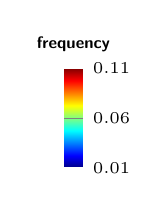
\begin{tikzpicture}
\begin{axis}[font=\bf\sffamily\fontsize{6}{6}\selectfont,
  hide axis,major tick length=0pt,
  xtick=\empty,
    scale only axis,
    height=0pt,
    width=0pt,
    colormap/jet,
    colorbar,
    point meta min=0.01,
    point meta max=0.11,
    colorbar style={title={frequency},title style={yshift=-.05in},font=\bf\sffamily\fontsize{6}{6}\selectfont,draw=none,axis line style={white}, y tick label style={
        /pgf/number format/.cd,
            fixed,
            fixed zerofill,
            precision=2,
        /tikz/.cd
    },  height=.5in,width=.1in,
        ytick={0.01,0.06,0.11}
    }]
    \addplot [draw=none] coordinates {(0,0)};
\end{axis}
\end{tikzpicture}};
  % \node[anchor=north west,label={[]90:{\large b.} 2018-2019 (Northern Hemisphere)}] (T2) at ([xshift=.1in]T1.south west) {
  %   \begin{tikzpicture}[font=\bf\sffamily\fontsize{7}{7}\selectfont]
  %     \node[] (A) at (0,0) {
  %       \mnp{2.65in}{\begin{texshade}{\SEQB}
  %           \shadingmode[chemical]{functional}
  %           \hideallmatchpositions
  %           \rulersteps{1}
  %           \setfont{residues}{sf}{up}{bf}{tiny} 
  %           \setfont{numbering}{sf}{up}{bf}{tiny} 
  %           \setfont{names}{tt}{up}{bf}{small}
  %           \setfont{legend}{tt}{up}{bf}{scriptsize}
  %           \threshold[80]{50}
  %           \setends{1}{1..\LENA}
  %           \showruler{1}{top}
  %           \hideconsensus
  %           \shadeallresidues
  %           \showlegend
  %         \end{texshade}
  %         % 
  %         \begin{texshade}{\SEQB}
  %           %\shadingmode[standard area]{functional}
  %           \shadingmode[hydropathy]{functional}
  %           \hideallmatchpositions
  %           \rulersteps{1}
  %           \setfont{residues}{sf}{up}{bf}{tiny} 
  %           \setfont{numbering}{sf}{up}{bf}{tiny} 
  %           \setfont{names}{tt}{up}{bf}{small}
  %           \setfont{legend}{tt}{up}{bf}{scriptsize}
  %           \threshold[80]{50}
  %           \setends{1}{1..\LENA}
  %           \showruler{1}{top}
  %           \hideconsensus
  %           \shadeallresidues
  %           \showlegend
  %         \end{texshade}
  %         % 
  %         \begin{texshade}{\SEQB}
  %           \shadingmode[accessible area]{functional}
  %           \hideallmatchpositions
  %           \rulersteps{1}
  %           \setfont{residues}{sf}{up}{bf}{tiny}
  %           \setfont{numbering}{sf}{up}{bf}{tiny} 
  %           \setfont{names}{tt}{up}{bf}{small}
  %           \setfont{legend}{tt}{up}{bf}{scriptsize}
  %           \threshold[80]{50}
  %           \setends{1}{1..\LENA}
  %           \showruler{1}{top}
  %           \hideconsensus
  %           \shadeallresidues
  %           \showlegend
  %         \end{texshade}
  %         % 
  %       }};
  %   \end{tikzpicture}};

 %  \node[anchor=north west,label={[]90:{\large c.} 2016-2017 (Southern Hemisphere)}] (T2) at ([xshift=0in]T1.south west) {
%     \begin{tikzpicture}[font=\bf\sffamily\fontsize{7}{7}\selectfont]
%       \node[ ] (A) at (0,0) {
%         \mnp{3.5in}{\begin{texshade}{\SEQC}
%             %\shadingmode[chemical]{functional}
%             \shadingmode[accessible area]{functional}
%             \hideallmatchpositions
%             \rulersteps{1}
%             \setfont{residues}{sf}{up}{bf}{tiny} 
%             \setfont{numbering}{sf}{up}{bf}{tiny} 
%             \setfont{names}{tt}{up}{bf}{small}
%             \setfont{legend}{tt}{up}{bf}{scriptsize}
%             \threshold[80]{50}
%             \setends{1}{1..\LENA}
%             \showruler{1}{top}
%             \hideconsensus
%             \shadeallresidues
%             \showlegend
%           \end{texshade}}};
% \node[] (B) at (A.north east) {  \mnp{3.5in}{      
%           % 
%           \begin{texshade}{\SEQC}
%             %\shadingmode[standard area]{functional}
%             \shadingmode[hydropathy]{functional}
%             \hideallmatchpositions
%             \rulersteps{1}
%             \setfont{residues}{sf}{up}{bf}{tiny} 
%             \setfont{numbering}{sf}{up}{bf}{tiny} 
%             \setfont{names}{tt}{up}{bf}{small}
%             \setfont{legend}{tt}{up}{bf}{scriptsize}
%             \threshold[80]{50}
%             \setends{1}{1..\LENA}
%             \showruler{1}{top}
%             \hideconsensus
%             \shadeallresidues
%             \showlegend
%           \end{texshade}}};


      
%     \end{tikzpicture}};


  

  % \node[anchor=north west,label={[]90:{\large d.} 2016-2017 (Northern Hemisphere)}] (T4) at ([xshift=0in]T3.south west) {
  %   \begin{tikzpicture}[font=\bf\sffamily\fontsize{7}{7}\selectfont]
  %     \node[label={[yshift=-1in,xshift=.15in]170:\mnp{.4in}{\raggedright type \\ \vspace{35pt} sd. chn. area \\ \vspace{35pt} acc. sd. chn.}}] (A) at (0,0) {
  %       \mnp{3.2in}{\begin{texshade}{\SEQD}
  %           \shadingmode[chemical]{functional}
  %           \hideallmatchpositions
  %           \rulersteps{1}
  %           \setfont{residues}{sf}{up}{bf}{tiny} 
  %           \setfont{numbering}{sf}{up}{bf}{tiny} 
  %           \setfont{names}{tt}{up}{bf}{small}
  %           \setfont{legend}{tt}{up}{bf}{scriptsize}
  %           \threshold[80]{50}
  %           \setends{1}{1..\LENA}
  %           \showruler{1}{top}
  %           \hideconsensus
  %           \shadeallresidues
  %           % \showlegend
  %         \end{texshade}
  %         % 
  %         \begin{texshade}{\SEQD}
  %           %\shadingmode[standard area]{functional}
  %           \shadingmode[hydropathy]{functional}
  %           \hideallmatchpositions
  %           \rulersteps{1}
  %           \setfont{residues}{sf}{up}{bf}{tiny} 
  %           \setfont{numbering}{sf}{up}{bf}{tiny} 
  %           \setfont{names}{tt}{up}{bf}{small}
  %           \setfont{legend}{tt}{up}{bf}{scriptsize}
  %           \threshold[80]{50}
  %           \setends{1}{1..\LENA}
  %           \showruler{1}{top}
  %           \hideconsensus
  %           \shadeallresidues
  %           % \showlegend
  %         \end{texshade}
  %         % 
  %         \begin{texshade}{\SEQD}
  %           \shadingmode[accessible area]{functional}
  %           \hideallmatchpositions
  %           \rulersteps{1}
  %           \setfont{residues}{sf}{up}{bf}{tiny}
  %           \setfont{numbering}{sf}{up}{bf}{tiny} 
  %           \setfont{names}{tt}{up}{bf}{small}
  %           \setfont{legend}{tt}{up}{bf}{scriptsize}
  %           \threshold[80]{50}
  %           \setends{1}{1..\LENA}
  %           \showruler{1}{top}
  %           \hideconsensus
  %           \shadeallresidues
  %           % \showlegend
  %         \end{texshade}
  %         % 
  %       }};
  %   \end{tikzpicture}};



  % \node[anchor=north west,label={[]90:{\large e.} 2016-2017 (H3N2 Northern Hemisphere)}] (T5) at ([xshift=0in]T4.south west) {
  %   \begin{tikzpicture}[font=\bf\sffamily\fontsize{7}{7}\selectfont]
  %     \node[label={[yshift=-1in,xshift=.15in]170:\mnp{.4in}{\raggedright type \\ \vspace{35pt} sd. chn. area \\ \vspace{35pt} acc. sd. chn.}}] (A) at (0,0) {
  %       \mnp{3.2in}{\begin{texshade}{\SEQE}
  %           \shadingmode[chemical]{functional}
  %           \hideallmatchpositions
  %           \rulersteps{1}
  %           \setfont{residues}{sf}{up}{bf}{tiny} 
  %           \setfont{numbering}{sf}{up}{bf}{tiny} 
  %           \setfont{names}{tt}{up}{bf}{small}
  %           \setfont{legend}{tt}{up}{bf}{scriptsize}
  %           \threshold[80]{50}
  %           \setends{1}{1..\LENA}
  %           \showruler{1}{top}
  %           \hideconsensus
  %           \shadeallresidues
  %           % \showlegend
  %         \end{texshade}
  %         % 
  %         \begin{texshade}{\SEQE}
  %           %\shadingmode[standard area]{functional}
  %           \shadingmode[hydropathy]{functional}
  %           \hideallmatchpositions
  %           \rulersteps{1}
  %           \setfont{residues}{sf}{up}{bf}{tiny} 
  %           \setfont{numbering}{sf}{up}{bf}{tiny} 
  %           \setfont{names}{tt}{up}{bf}{small}
  %           \setfont{legend}{tt}{up}{bf}{scriptsize}
  %           \threshold[80]{50}
  %           \setends{1}{1..\LENA}
  %           \showruler{1}{top}
  %           \hideconsensus
  %           \shadeallresidues
  %           % \showlegend
  %         \end{texshade}
  %         % 
  %         \begin{texshade}{\SEQE}
  %           \shadingmode[accessible area]{functional}
  %           \hideallmatchpositions
  %           \rulersteps{1}
  %           \setfont{residues}{sf}{up}{bf}{tiny}
  %           \setfont{numbering}{sf}{up}{bf}{tiny} 
  %           \setfont{names}{tt}{up}{bf}{small}
  %           \setfont{legend}{tt}{up}{bf}{scriptsize}
  %           \threshold[80]{50}
  %           \setends{1}{1..\LENA}
  %           \showruler{1}{top}
  %           \hideconsensus
  %           \shadeallresidues
  %           % \showlegend
  %         \end{texshade}
  %         % 
  %       }};
  %   \end{tikzpicture}};


  
\end{tikzpicture}  
  \vspace{0pt}   
  
  \else
  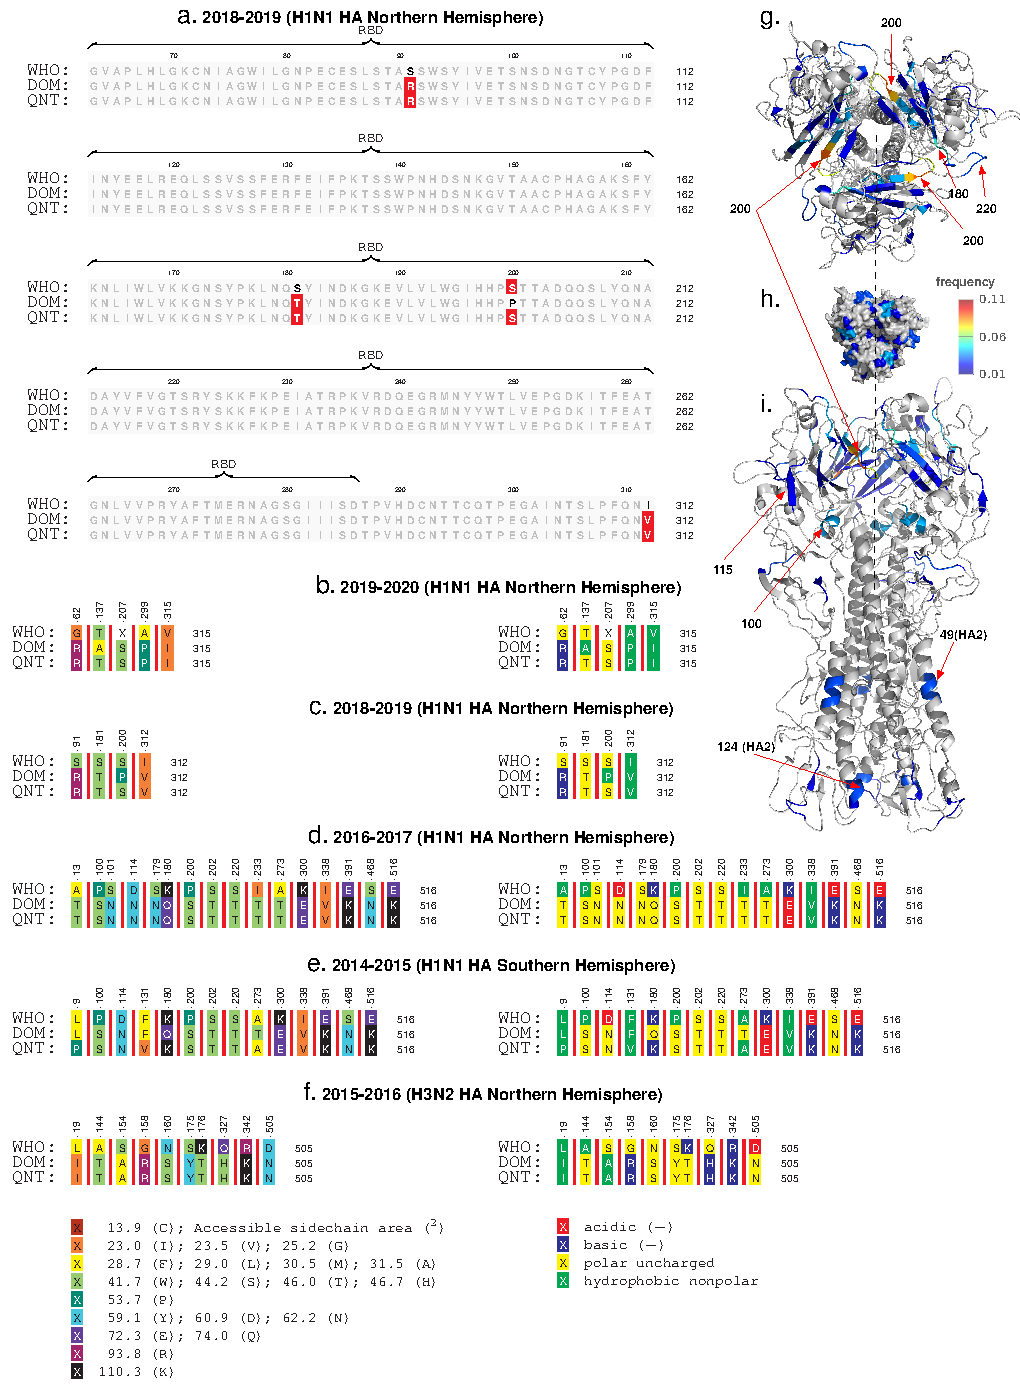
\includegraphics[width=0.87\textwidth]{Figures/External/sequence.pdf}  \vspace{-5pt}   

  \fi
\vspace{0pt}

\captionN{\textbf{Sequence comparisons.} The observed dominant strain, we note that the correct \qnet  deviations tend to be within the RBD, both for H1N1 and H3N2 for HA (panel a shows one example). Additionally, by comparing the type, side chain area, and the accessible side chain area, we note that the changes often have very different properties (panel b-f). Panels g-i show the localization of the deviations in the molecular structure of HA, where we note that the changes are most frequent in the HA1 sub-unit (the globular head), and around residues and structures that have been commonly implicated in receptor binding interactions $e.g$ the $\approx 200$ loop, the $\approx 220$ loop and the $\approx 180$-helix.}\label{figseq}
\end{figure*}
\else
\refstepcounter{figure}\label{figseq}
\fi
%#############################################
%#############################################


%#############################################
%#############################################

\begin{table}\centering
\captionN{Riskiest Strains Currently Circulating in Swine}\label{tabrec11}

\sffamily\fontsize{7}{8}\selectfont

\begin{tabular}{L{2.1in}|L{0.7in}|L{0.7in}|L{0.7in}}\hline
 \rowcolor{lightgray}H1N1 Strain & HA Risk & NA Risk & Overall Risk \\\hline
 A/swine/Tennessee/A02524414/2022 &0.0201&0.0030&0.0077\\\hline
 A/swine/Missouri/A02750646/2022 &0.0201&0.0070&0.0118\\\hline
 A/swine/Kansas/A02711847/2022 &0.0201&0.0098&0.0141\\\hline
 A/swine/Iowa/A02636572/2022 &0.0166&0.0225&0.0193\\\hline
 A/swine/Iowa/A02636308/2021 &0.0143&0.0266&0.0195\\\hline
 A/swine/Illinois/A02750711/2022 &0.0166&0.0233&0.0197\\\hline
 A/swine/Iowa/A02636616/2022 &0.0166&0.0233&0.0197\\\hline
 A/swine/Oklahoma/A02246915/2022 &0.0166&0.0233&0.0197\\\hline
 A/swine/Colorado/A02636469/2022 &0.0166&0.0233&0.0197\\\hline
 A/swine/Iowa/A02636297/2021 &0.0149&0.0267&0.0200\\\hline
 \rowcolor{lightgray}H3N2 Strain & HA Risk & NA Risk & Overall Risk \\\hline
 A/swine/Indiana/A02636492/2022 &0.0104&0.0113&0.0108\\\hline
 A/swine/Indiana/A02636512/2022 &0.0104&0.0113&0.0108\\\hline
 A/swine/Iowa/A02750695/2022 &0.0110&0.0120&0.0115\\\hline
 A/swine/Oklahoma/A02711859/2022 &0.0122&0.0114&0.0118\\\hline
 A/swine/Iowa/A02636351/2022 &0.0121&0.0119&0.0120\\\hline
 A/swine/Iowa/A02636476/2022 &0.0121&0.0120&0.0121\\\hline
 A/swine/Texas/A02636569/2022 &0.0122&0.0120&0.0121\\\hline
 A/swine/Iowa/A02750726/2022 &0.0123&0.0120&0.0121\\\hline
 A/swine/Iowa/A02750740/2022 &0.0104&0.0156&0.0127\\\hline
 A/swine/Indiana/A02636521/2022 &0.0104&0.0156&0.0127\\\hline
 \end{tabular}
\flushleft

\fontsize{7}{7}\selectfont
$^\star$ Converted IRAT Score computed using regression generated from the IRAT vs. Qnet comparison
\end{table}
%#############################################
%#############################################




